\documentclass[12pt,a4paper]{article}
\usepackage[polish]{babel}
\usepackage[T1]{fontenc}
\usepackage{hyperref}
\usepackage{url}
\usepackage{graphicx}
\graphicspath{ {images/} }
\usepackage{csquotes}
\usepackage[utf8x]{inputenc}


\addtolength{\hoffset}{-1.5cm}
\addtolength{\marginparwidth}{-1.5cm}
\addtolength{\textwidth}{3cm}
\addtolength{\voffset}{-1cm}
\addtolength{\textheight}{2.5cm}
\setlength{\topmargin}{0cm}
\usepackage{algorithm}
\usepackage[noend]{algpseudocode}
\setlength{\headheight}{0cm}

\begin{document}
    \begin{titlepage}
       \begin{center}
           \vspace*{1cm}
           
           {\fontsize{23}{25}\selectfont Dokumentacja projektu\\Systemy sztucznej inteligencji}
     
            \vspace{1.0cm}
        
            {\fontsize{17}{18}\selectfont Dawid Bitner \\ Daniel Broczkowski \\ Mateusz Kowol \\ Marcin Krupa}
           
            \vspace{0.4cm}
           
            {\fontsize{12}{13}\selectfont 6 czerwca 2019}
           
            \vfill
            \vspace{0.8cm}
     
            {\fontsize{13}{14}\selectfont Politechnika Śląska\\Wydział Matematyki Stosowanej\\Rok akademicki 2018/2019}
     
       \end{center}
    \end{titlepage}
	\newpage
	\tableofcontents
	\newpage
	\section{Część I}
	\subsection{Opis programu}

	Program \textit{Meowfinder} jest realizacją projektu z przedmiotu \textit{Systemy sztucznej inteligencji}, polegającym na klasyfikacji obrazów z wykorzystaniem sieci konwolucyjnych. Program realizuje klasyfikację zwierząt na podstawie obrazu przekazanego do sieci. Wynikiem jest rozpoznanie i przypisanie zwierzęcia do jednej z klas, według odpowiednio wcześniej posegregowanych zdjęć, które przedstawiają różne rodzaje i gatunki zwierząt, tj.: psy, koty, konie, małpy, pająki, motyle, krowy, kury, słonie, wiewiórki, krowy oraz owce.\\\\
	Projekt został opracowany w języku Python, wykorzystując bibliotekę do nauczania maszynowego \textit{Tensorflow}, a w niej \textit{TFlearn}, z którego pomocą został zbudowany model sieci CNN.
	\subsection{Instrukcja obsługi}

	Aby uruchomić program, należy mieć zainstalowany pakiet bibliotek oraz opcjonalnie środowisko programistyczne (PyCharm, Anaconda). Plik główny to \textit{main.py}. Po jego uruchomieniu włączy nam się konsola z możliwością wyboru jednej z trzech opcji.
	\begin{center}
        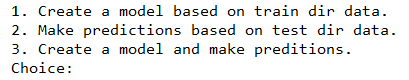
\includegraphics[scale=1]{1.png}
        \begin{flushright}
            \begin{scriptsize}
            Menu opcji z konsoli.
            \end{scriptsize}
        \end{flushright}
    \end{center}
	1) Program tworzy model, bazując na plikach zdjęć z folderu \textit{train}. W folderze powinny znajdować się podfoldery z fotografiami zwierząt, odpowiednio sklasyfikowane poprzez nazwanie ich odpowiadającym zwierzętom gatunkom.
	\begin{center}
        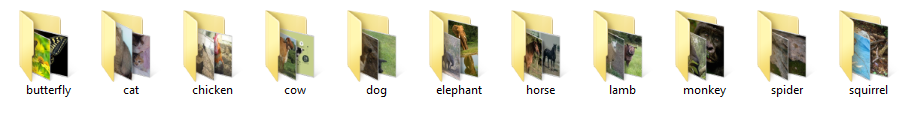
\includegraphics[scale=0.6]{3.png}
        \begin{flushright}
            \begin{scriptsize}
            Prawidłowa zawartość folderu train.
            \end{scriptsize}
        \end{flushright}
    \end{center}
	Następnie zdjęcia te zostają przetworzone i zapisane w pliku \textit{train\_data.npy}.
	\begin{center}
        
\includegraphics[scale=1]{2.png}
        \begin{flushright}
            \begin{scriptsize}
            Menu opcji z konsoli.
            \end{scriptsize}
        \end{flushright}
    \end{center}
    Po zakończonym procesie nauki zostają utworzone pliki modelu:
    \begin{center}
        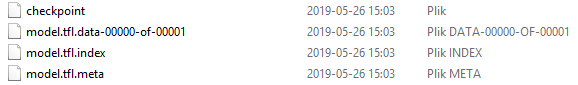
\includegraphics[scale=1]{4.png}
        \begin{flushright}
            \begin{scriptsize}
            Przykładowe pliki modelu.
            \end{scriptsize}
        \end{flushright}
    \end{center}
    
	2) Program, na podstawie zdjęć znajdujących się w folderze, \textit{test} przewiduje, które ze zwierząt znajduje się na fotografii oraz z jaką skutecznością zostało to określone. Wyniki 20 fotografii zostają przedstawione w wyświetlonym oknie na wykresie.
	\begin{center}
        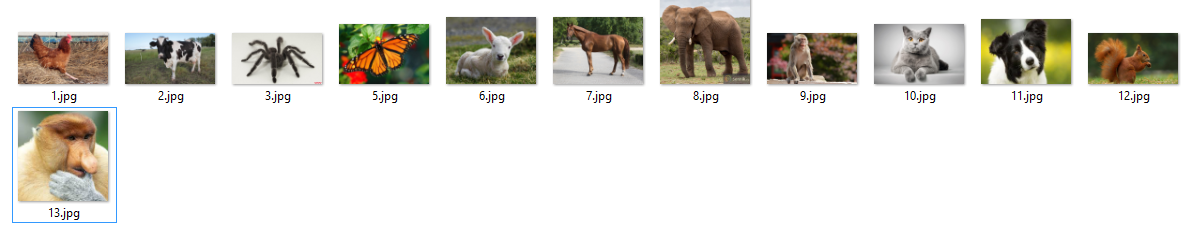
\includegraphics[scale=0.5]{5.png}
        \begin{flushright}
            \begin{scriptsize}
            Prawidłowa zawartość folderu test.
            \end{scriptsize}
        \end{flushright}
        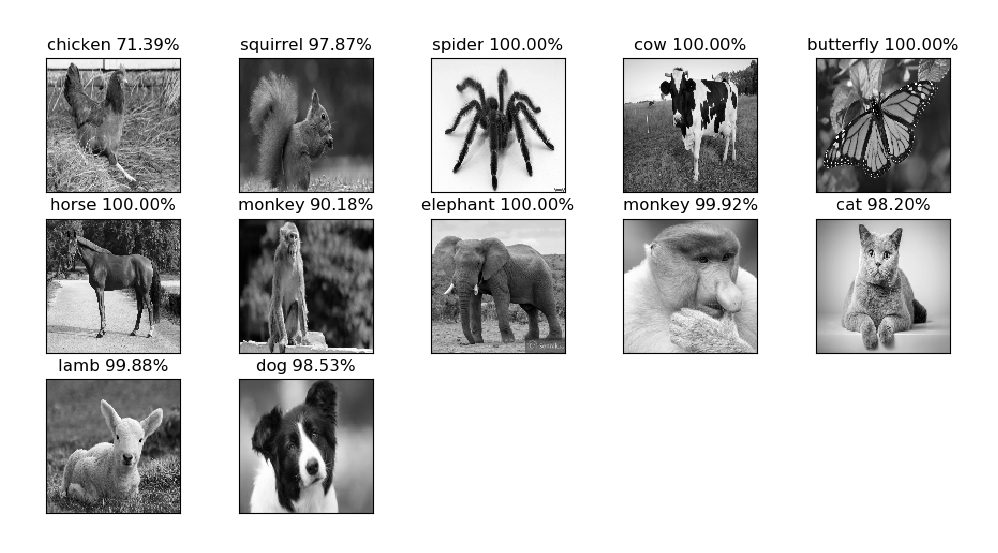
\includegraphics[scale=0.6]{6.png}
        \begin{flushright}
            \begin{scriptsize}
            Przewidywania sieci zapisane na wykresie.
            \end{scriptsize}
        \end{flushright}
    \end{center}
	3) Uruchomi poprzednie punkty jeden po drugim
	
\newpage
	\section{Część II}
	\subsection{Część techniczna}
	Struktura projektu podzielona jest na odrębne pliki, które realizują określone funkcje i działania:
	\begin{enumerate}
        	\item \textit{Main} - zawiera menu wraz z opcjami. Zawiera klasę Switcher, która wywołuje odpowiednie metody do prawidłowego działania programu. Funkcje wewnątrz klasy Switcher:
        	\begin{itemize}
        	    \item \textit{decision} - konstruktor, przyjmuje decyzję użytkownika.
        	    \item \textit{createModel} - wywołuje funkcje związane z tworzeniem modelu.
        	    \item \textit{makePredictions} - wywołuje funkcje związane z określeniem przynależności.
        	    \item \textit{both} - wywołuje obie metody wewnątrz klasy.
        	\end{itemize}
        	\item \textit{Settings} - plik, przechowujący dane dotyczące m.in. ścieżek do folderów \textit{train} oraz \textit{test}, preferowanego rozmiaru obrazka przez sieć czy listę z klasami zwierząt.
        	\item \textit{Train\_data} - plik z funkcją, realizującą zapis zdjęć z folderu \textit{train}, wraz z odpowiednimi etykietami dla klas, do listy wypełnionej krotkami. Krotka zawiera macierz RGB w odcieniach szarości oraz listę z przynależnością zwierzęcia na obrazku zakodowaną za pomocą 11-wymiarowego wektora, tzw. one hot-enconding. W celu zamiany zdjęcia na skalę szarości, funkcja używa biblioteki \textit{OpenCV} dla przyśpieszenia procesu. Wykorzystując bibliotekę \textit{NumPy}, zrealizowaliśmy zapis listy krotek do pliku \textit{train\_data.npy} o rozszerzeniu \textit{.npy}, charakterystycznym dla tej biblioteki. Zapis macierzy RGB nie jest normalizowany na tym etapie.
        	\item \textit{Test\_data} - realizuje podobne zadania, jak funkcje z pliku \textit{Train\_data}, różnica jest w operowaniu na folderze \textit{test}, gdzie użytkownik zadaje zdjęcia do określenia ich przynależności. Tablica RGB w odcieniach szarości zapisywana jest do pliku \textit{test\_data.npy}
        	\item \textit{Neural\_network} - plik z modelem sieci CNN, realizującym naukę. Na start realizowany jest podział plików zapisanych w pliku \textit{train\_data.npy} na pliki do treningu oraz walidacji. Dane te są normalizowane do wartości z przedziału $[0; 1]$ aby przeprowadzić tzw. zero-centering, czyli liniową transformację danych, która przesuwa dane tak, aby były skoncentrowane na początku. Kolejnym etapem jest realizacja nauki poprzez zbudowany model sieci CNN z użyciem biblioteki \textit{TFlearn} pakietu \textit{TensorFlow}. Jeśli istniał model, przed nauką wczytywane są wagi w celu dalszego rozwijania sieci. Po zakończonym procesie nauki, model zapisywany jest do folderu głównego aplikacji.
        	\item \textit{Plot\_data} - plik, realizujący proces przewidywania przez sieć wyników na podstawie danych zapisanych w pliku \textit{test\_data.npy}. Zawiera on model sieci CNN identyczny jak ten, wykorzystany w procesie nauki, przez który przechodzą zdjęcia do testów. Wynik wypisywany jest na wykresie wraz z pewnością, z jaką sieć była w stanie określić przynależność zwierzęcia do jednej z klas. Zawiera dwie funkcje:
        	\begin{itemize}
        	    \item \textit{cnn} - kopia modelu z pliku \textit{Neural\_network}.
        	    \item \textit{plt\_dat} - funkcja, realizująca wypisywanie na grafie.
        	\end{itemize}
    	\end{enumerate}
    Jeśli wybierzemy opcję nr 3 z menu opcji, program będzie realizowany przez funkcję main w kolejności:\\
    1). Stworzenie danych do nauki na podstawie folderu \textit{train}, wykorzystując funkcje z pliku \textit{Train\_data}.\\
    2). Budowanie modelu, wykorzystując funkcje z pliku \textit{Neural\_network}.\\
    3). Stworzenie danych testowych, wykorzystując funkcje z pliku \textit{Test\_data}.\\
    4). Proces przewidywania, realizowany przez funkcje z pliku \textit{Plot\_data}.
	
	\subsection{Opis działania}
	
    Do klasyfikacji zwierząt wykorzystano konwolucyjną sieć neuronową. Jej największą zaletą jest wykrywanie i uczenie się hierarchicznie cech, tj. tych, które są warte uwagi, i jak je przetwarzać bez nadzoru człowieka. Są one podobne w budowie do zwykłych sieci neuronowych - posiadają neurony, które mają swoje wagi i odchylenia (bias), neurony otrzymują dane wejściowe i wykonują obliczenia w postaci iloczynów skalarnych, które traktują nieliniową funkcją aktywacyjną. Potrafią sklasyfikować zdjęcia na podstawie pikseli z otrzymanego obrazka, posiadają funkcję straty (minimalizująca odchylenie wartości obserwowanej od przewidywanej) na ostatniej w pełni połączonej warstwie.
    \\
    
    Znaczącą różnicą jest to, że sieci ConvNet zostały zaprojektowane do przetwarzania obrazów i obiektów, które się na nich znajdują. Dzięki zastosowaniu odpowiednich filtrów, łatwiej jest im uchwycić zależności przestrzenne na obrazie. Pre-processing wymagany w sieciach typu ConvNet jest znacznie niższy, w porównaniu z innymi algorytmami klasyfikacji. Architektura zapewnia lepsze dopasowanie do zestawu danych, składających się z obrazów, dzięki zmniejszeniu liczby zaangażowanych parametrów i możliwości ponownego użycia wag, przez co funkcja przekazywania jest bardziej wydajna w implementacji. 
    \\
    
    Przykład: pierwsza ukryta warstwa w normalnej sieci neuronowej, gdzie dane wejściowe to obrazy. Jeśli obraz ma rozmiar 128x128x3, gdzie 3 oznacza liczbę kanałów (np. RGB), pierwsza warstwa będzie miała 49152 wag. Pełne łączenie warstw w tym przypadku jest bezsensowne, a ogromna liczba parametrów doprowadzi tylko do overfittingu sieci.
    \begin{center}
        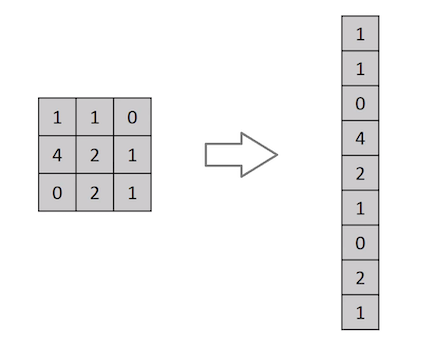
\includegraphics[scale=0.5]{input_vector.png}
        \begin{flushright}
            \begin{scriptsize}
            Przykładowa warstwa wejściowa dla klasycznego modelu sieci, obraz 3x3 odcieniach szarości z jedną warstwą głębi.
            \end{scriptsize}
        \end{flushright}
    \end{center}
    
    Architektura sieci ConvNet składa się z kilku warstw, które przekształcają oryginalny obraz warstwa po warstwie do wartości potrzebnych do klasyfikacji:
    \begin{itemize}
        \item Warstwa wejściowa
        \item Warstwy konwolucyjne
        \item Warstwa aktywacji
        \item Max-pooling
        \item Fully-connected
    \end{itemize}
    \subsubsection{Warstwa wejściowa}
    
    W sieci ConvNet, gdzie na wejście podajemy obraz, neurony są ułożone w trzech wymiarach: szerokości, wysokości i głębi. Neurony w warstwie zostaną połączone tylko z małym obszarem warstwy poprzedniej zamiast pełnego łączenia. Warstwa wyjściowa zmniejszy pełny obraz do pojedynczego wektora klasyfikacji, rozmieszczonego wzdłuż wymiaru głębi. Ważne jest zredukowanie obrazów do postaci łatwiejszej do przetworzenia, bez utraty cech, które są kluczowe dla uzyskania dobrego wyniku. Ważne jest, by nasza architektura skalowała się do ogromnych zbiorów danych.
    \begin{center}
        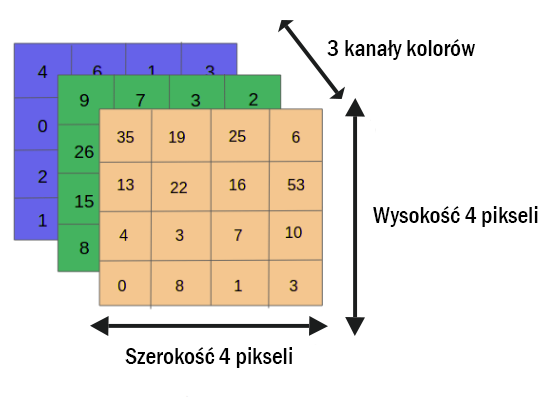
\includegraphics[scale=0.5]{input.png}
        \begin{flushright}
            \begin{scriptsize}
            Przykład danych wejściowych w postaci obrazka w sieci ConvNet.
            \end{scriptsize}
        \end{flushright}
    \end{center}
    \subsubsection{Warstwy konwolucyjne}
        \begin{center}
            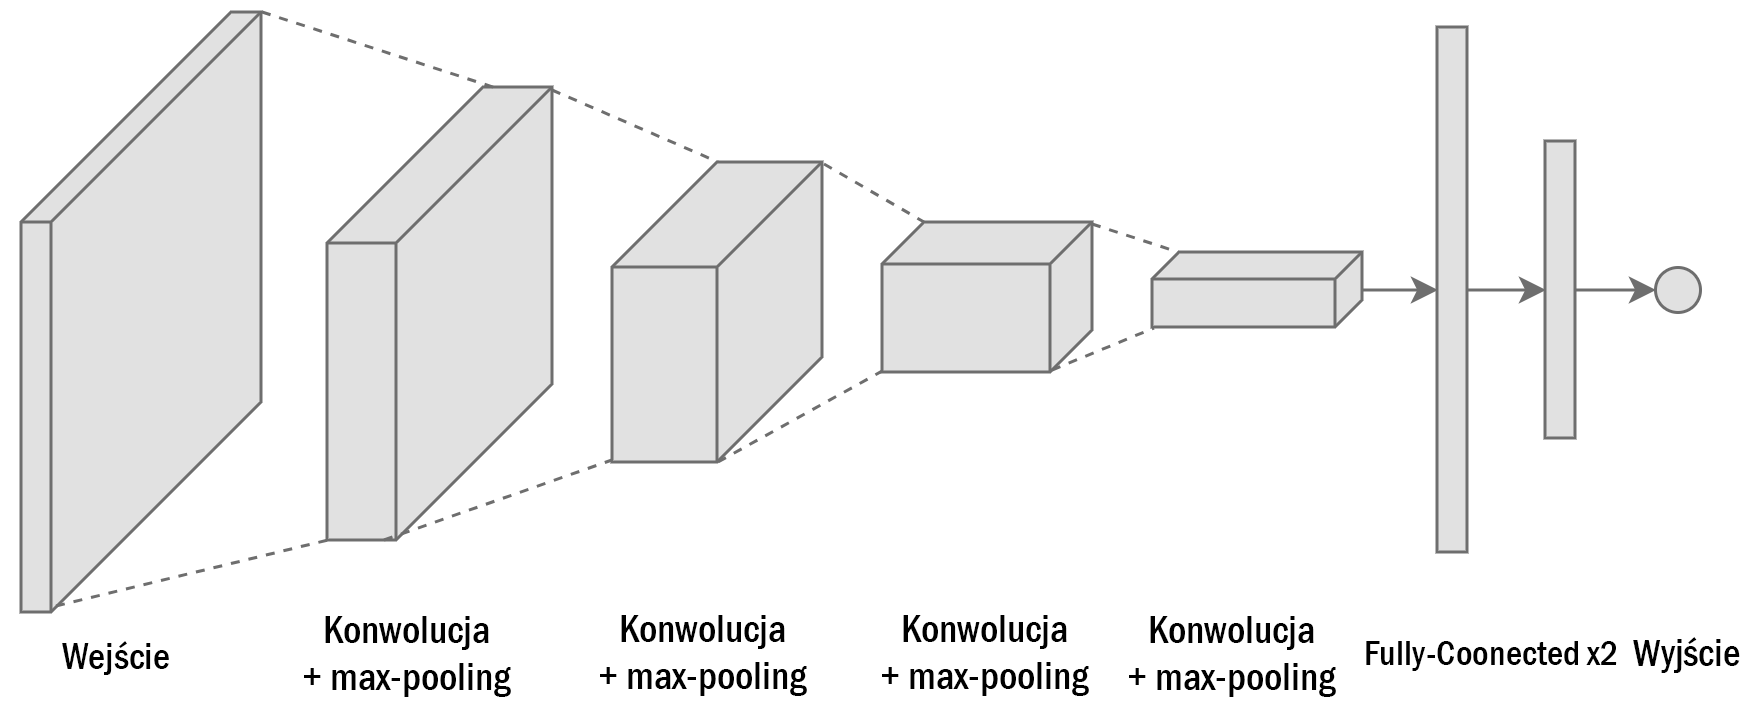
\includegraphics[scale=0.2]{dudi.png}
            \begin{flushright}
                \begin{scriptsize}
                Przykład logistyczny sieci typu ConvNet.
                \end{scriptsize}
            \end{flushright}
        \end{center}
        
        Główny blok sieci CNN. Zawierają zestaw filtrów, które podlegają nauce. Splot (ang. Convolution) jest operacją matematyczną, służącą do scalenia dwóch funkcji, tworząc nową - trzecią. W przypadku sieci, gdzie wejściem jest obraz, splot jest stosowany na danych wejściowych za pomocą filtra splotowego (kernel), aby utworzyć mapę cech  (feature map).
        \\
        
        Dokonujemy splotu, przesuwając filtr na wejściu. Przeprowadzane jest mnożenie macierzy, a suma zapisywana jest na mapę cech.
        \begin{center}
            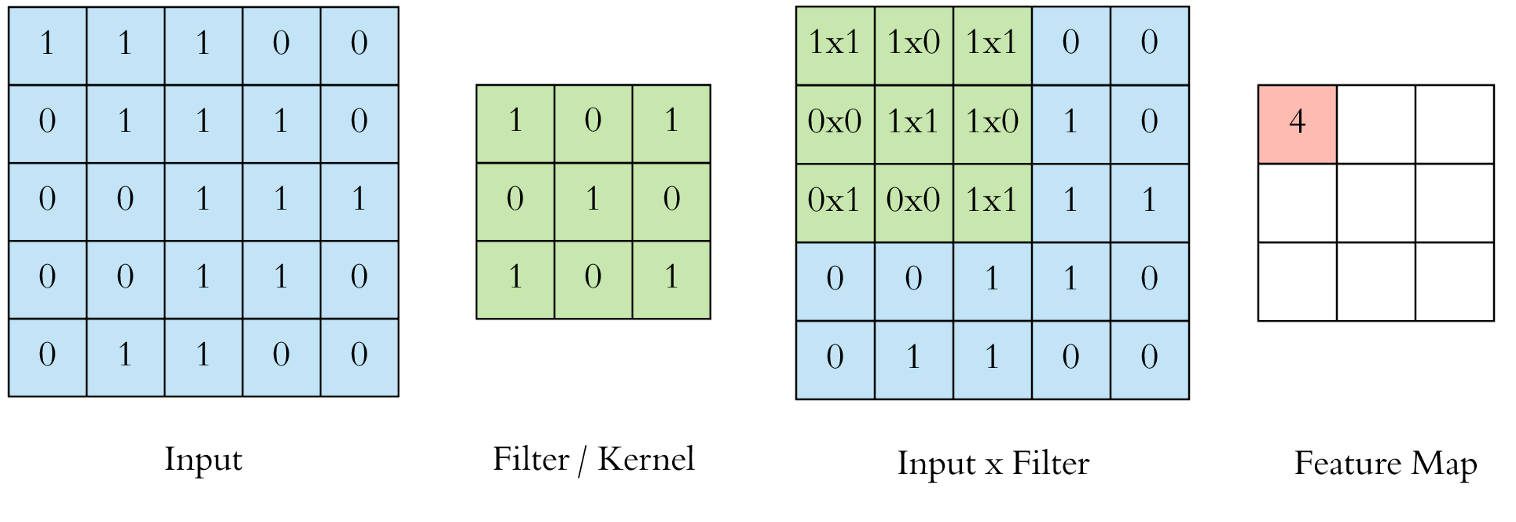
\includegraphics[scale=0.35]{kernel.png}
            \begin{flushright}
                \begin{scriptsize}
                Przykładowy filtr 3x3 oraz dane wejściowe na danych 2D. Filtr (zielony kwadrat) przesuwa się po wejściu (niebieski kwadrat), a suma splotu przechodzi do mapy cech (czerwony kwadrat).
                \end{scriptsize}
            \end{flushright}
        \end{center}
        
        Powyższy przykład jest wykonany w 2D. W sieciach ConvNet sploty dokonywane są w 3D. Obraz reprezentowany jest jako matryca 3D o trzech wymiarach: wysokości, szerokości i głębi, gdzie głębia reprezentuje kanały RGB. Stosowany filtr na obrazie także musi być 3D, ponieważ musi pokryć całą głębię wejścia.
        \\
        
        Na wejściu dokonywane jest  wiele splotów, a każde z nich używa innego filtru i skutkuje odrębną mapą cech. Następnie połączenie tych wszystkich map cech staje się naszym końcowym wynikiem warstwy splotu.
        \begin{center}
            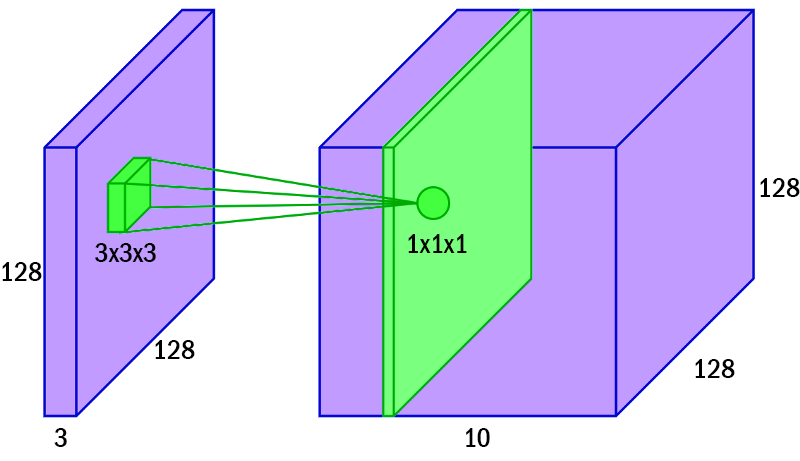
\includegraphics[scale=0.35]{3dkernel.png}
        \end{center}
        
        Generalnie, celem splotu jest wydobycie z obrazu wejściowego cech, takich jak krawędzie. ConvNets nie muszą być ograniczone tylko do jednej warstwy konwolucji. Tradycyjnie pierwszy ConvLayer jest odpowiedzialny za przechwytywanie cech, takich jak: krawędzie, kolor, orientacja gradientu itp., a dzięki dodawaniu kolejnych warstw można dostroić architekturę. Zyskujemy wtedy sieć, która  rozumie obrazy podobnie do nas.
        \\
        
        Przykład: obraz 128x128x3, kernel ma rozmiar 5x5x3. Gdy filtr znajduje się w określonym miejscu i obejmuje niewielki obszar wejścia, wykonujemy operację splotu z tą różnicą, że odbywa się to w trzech wymiarach. Wynikiem w dalszym ciągu jest skalar. Przesuwając filtr, obliczamy kolejne wartości zapisywane na mapie cech o rozmiarze 128x128x1. Rozmiar nie ulega zmianie dzięki zastosowaniu paddingu. Stosujemy go, jeśli chcemy zachować tę samą wymiarowość. Wtedy trzeba otoczyć wejście zerami. Gdybyśmy użyli 10 różnych filtrów, mielibyśmy 10 map cech o rozmiarze 128x128x1. Układając je wzdłuż wymiaru głębokości, dałyby nam końcowy wynik warstwy splotu: objętość o wymiarach 32x32x10. Operacja splotu dla każdego filtru jest wykonywana niezależnie, a wynikowe mapy cech są rozłączne. W projekcie zastosowano znacznie więcej filtrów w każdej warstwie.
        \begin{center}
            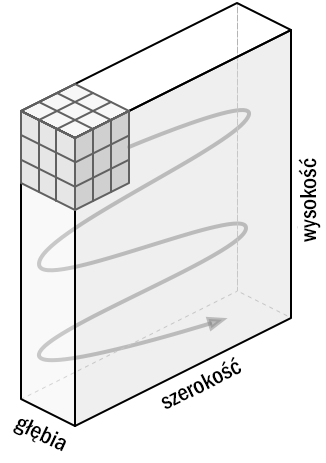
\includegraphics[scale=0.35]{kernel-movement.png}
            \begin{flushright}
                \begin{scriptsize}
                Przesuwanie kernela na obrazku.
                \end{scriptsize}
            \end{flushright}
        \end{center}
    \subsubsection{Warstwa aktywacji}
    
        Sieć CNN nie jest wyjątkiem, jeśli chodzi o użycie funkcji aktywacji pomiędzy warstwami. Projekt korzysta z funkcji ReLU do przekazywania wyniku operacji splotu. Używając funkcji aktywacji trzeba pamiętać o tym, że wartości w końcowych mapach cech nie są w rzeczywistości sumami, ale wartościami po zastosowaniu do nich funkcji aktywacji, oraz że każdy rodzaj splotu wymaga funkcji aktywacji, bez której sieć nie osiągnie swojego pełnego potencjału.
        Wzór ReLU:
        $$R(z)=max(0, z)$$
        $$z=Wx + b$$
        \begin{center}
            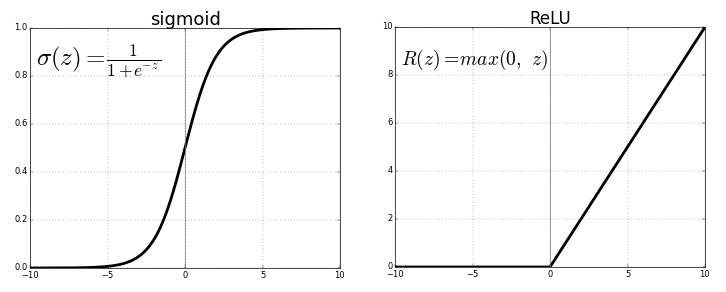
\includegraphics[scale=0.35]{act_graph.png}
            \begin{flushright}
                \begin{scriptsize}
                Porównanie ReLU z funkcją Sigmoid.
                \end{scriptsize}
            \end{flushright}
        \end{center}
        Wybór padł na ReLU z kilku powodów: zmniejszone prawdopodobieństwo zaniku gradientu (zmiana kierunku intensywności lub koloru obrazu), bardziej wydajny obliczeniowo do obliczania niż funkcje typu sigmoid (ReLU musi tylko wybrać $max(0, z)$, nie wykonuje przy tym kosztownych operacji wykładniczych).
    \subsubsection{Strides, max-pooling, padding}
    
    Strides: określa, o ile przesuwamy filtr splotu w każdym kroku. Możemy decydować o ile pozycji chcemy przesuwać filtr na każdym kroku - jeśli wartość jest duża, to wynikowa mapa cech jest mniejsza, ponieważ pomijamy potencjalne lokalizacje.
    \begin{center}
        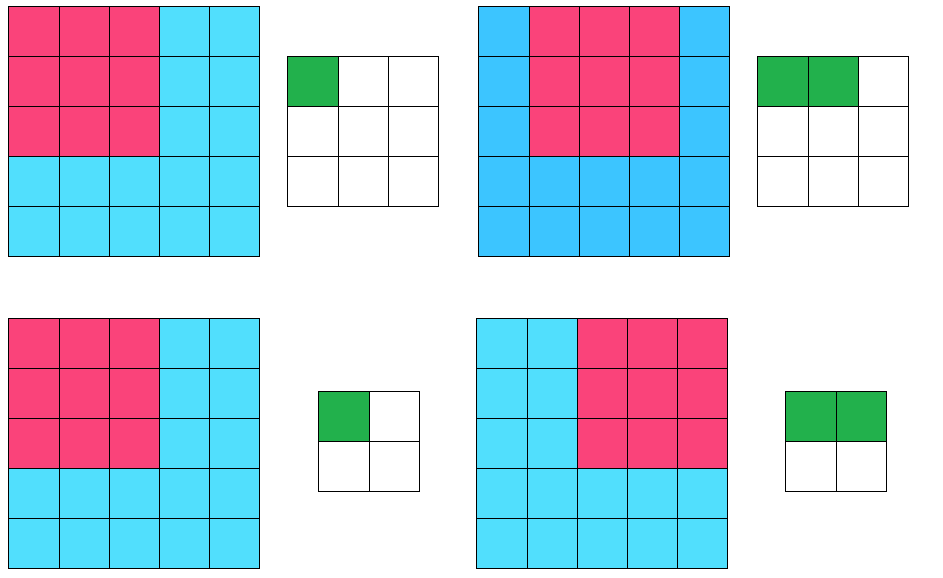
\includegraphics[scale=0.55]{stride_comparison.png}
        \begin{flushright}
            \begin{scriptsize}
            Porównanie strides ustawiony na wartość 1, oraz na wartość 2.
            \end{scriptsize}
        \end{flushright}
    \end{center}
    
    Stosując tę technikę, rozmiar mapy cech jest mniejszy niż wejście, ponieważ filtr splotu musi być zawarty w danych wejściowych. Jeśli chcemy zachować tę samą wymiarowość, możemy użyć \textit{paddingu}, aby otoczyć wejście zerami lub wartościami, które znajdują się na krawędzi (szary obszar wokół wejścia). Jest to powszechnie stosowana technika, aby zachować rozmiar map cech tak, aby zapobiec kurczeniu się na każdej warstwie. Tak samo jak na obrazku w 2D, używamy ich na warstwach kowolucyjnych, które są w 3D.
    \begin{center}
        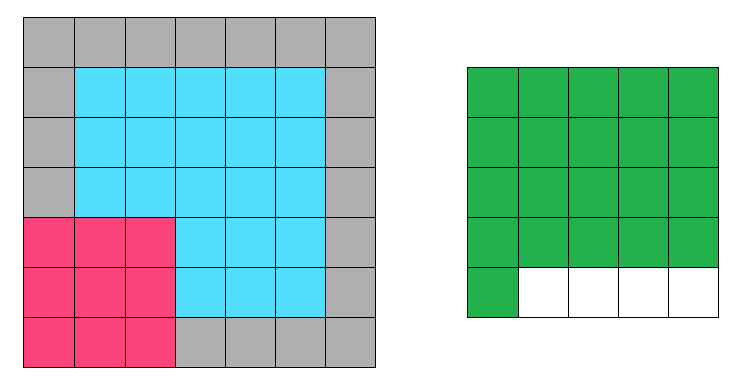
\includegraphics[scale=0.55]{padding.png}
        \begin{flushright}
            \begin{scriptsize}
            Wykorzystanie paddingu.
            \end{scriptsize}
        \end{flushright}
    \end{center}
    
    Kolejnym etapem jest tzw. \textit{pooling}. Technika ta redukuje "wymiarowość", dzięki czemu możemy zmniejszyć liczbę parametrów, co zarówno skraca czas szkolenia, jak i zwalcza nadmierne dopasowanie. Przy dużych sieciach, technika ta potrafi zredukować o kilkadziesiąt procent liczbę wag pomiędzy warstwami. Łączenie warstw w dół każdej mapy cech jest niezależne, zmniejsza wysokość i szerokość, zachowując przy tym nienaruszoną głębokość.
    \\
    
    Zwykle używa się tzw. max-pooling, które pobiera wartość maksymalną w oknie operacji. Operacja ta nie ma parametrów, po prostu okno operacji przesuwa się nad wejściem i  pobiera maksymalną wartość. Rozmiar okna i stride są jasno określone.
    \begin{center}
        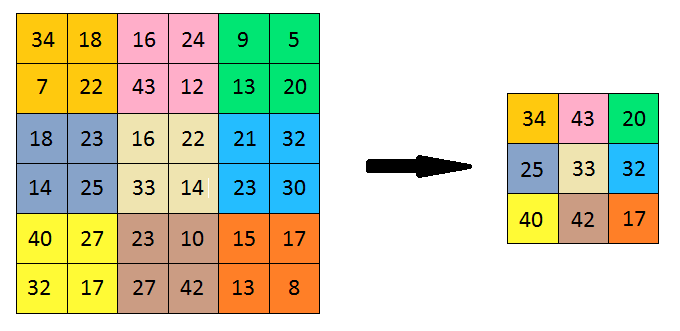
\includegraphics[scale=0.52]{max-pool.png}
        \begin{flushright}
            \begin{scriptsize}
            Max-pooling dla okna 2x2 i stride 2. Każdy kolor oznacza inne okno. Konfiguracja ta zmniejsza mapę cech o połowę.
            \end{scriptsize}
        \end{flushright}
    \end{center}
    
    \subsubsection{Hiperparametry}
    
    Czyli parametry, które powinniśmy przemyśleć przy tworzeniu sieci ConvNet. Zaliczamy do nich:
    \begin{itemize}
        \item Rozmiar filtru - jeśli jest mniejszy, wyodrębnianych jest więcej szczegółowych informacji z obrazka, które mogą być użyte później (działa to też w drugą stronę: mogą być wyodrębniane kompletnie nieprzydatne informacje), spowalnia zmniejszenie wymiaru obrazu. Większe filtry wyodrębniają dość ogólne cechy na obrazie, ilość wyodrębnionych informacji jest znacznie mniejsza. Szybka redukcja wymiaru obrazu sprawia, że sieć jest płytka.
        \item Liczba filtrów - najbardziej zmienny parametr w sieci CNN, zwykle jest to wartość pomiędzy 32 a 1024. Używanie większej liczby filtrów daje mocniejszy model, ale ryzykujemy przeładowanie z powodu zwiększonej liczby parametrów. Zwykle zaczynamy od małej liczby filtrów w początkowych warstwach i stopniowo zwiększamy liczbę, gdy wchodzimy głębiej w sieć.
        \item Stride
        \item Padding
    \end{itemize}
    \subsubsection{Fully-connected}
    
        Po operacjach splotu i max-poolingu dodajemy kilka w pełni połączonych warstw (fully-connected), aby zakończyć architekturę CNN. Warstwy te na wejście wymagają wektora 1D liczb, natomiast warstwy splotu jak i poolingu mają wektor 3D. Zatem musi nastąpić spłaszczenie (ang. \textit{flattening}).
        \\
        
        Spłaszczony sygnał wyjściowy jest podawany do sieci neuronowej i tak, jak w klasycznej sieci, stosowana jest wsteczna propagacja stosowana do każdej iteracji. Po serii epok, model jest w stanie rozróżniać dominujące i  nieistotne cechy w obrazach i klasyfikować je za pomocą techniki klasyfikacji \textit{Softmax}.
        \\
        
        Funkcja Softmax zamienia liczby na prawdopodobieństwa, które sumują się do jednego. Funkcja ta wyprowadza wektor, który reprezentuje rozkłady prawdopodobieństwa listy potencjalnych wyników.
        
        \begin{center}
            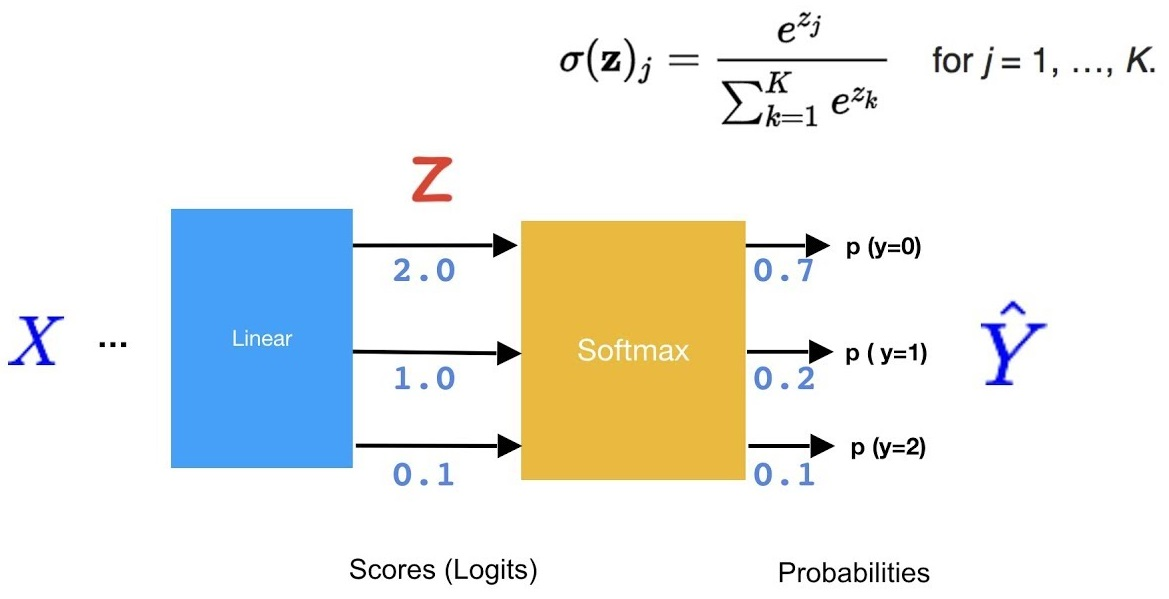
\includegraphics[scale=0.45]{softmax.png}
        \end{center}
    \subsubsection{Dropout}
        \begin{center}
            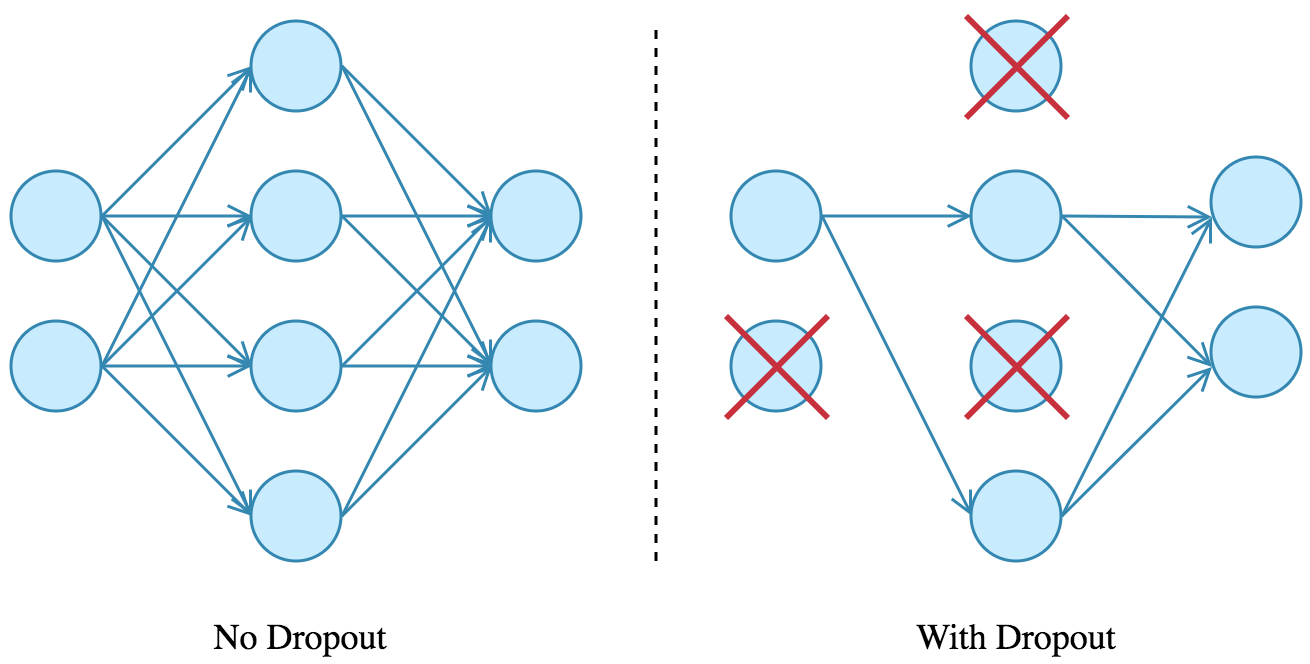
\includegraphics[scale=0.34]{dropout.png}
        \end{center}
        
        Dropout służy do zapobiegania przeuczeniu. Podczas treningu w każdej iteracji neuron jest tymczasowo „upuszczany” lub wyłączany z prawdopodobieństwem \textit{p}. Oznacza to, że wszystkie wejścia i wyjścia do tego neuronu zostaną wyłączone przy bieżącej iteracji. Porzucone neurony są poddawane ponownemu próbkowaniu z prawdopodobieństwem \textit{p} na każdym kolejnym kroku treningowym, więc porzucony neuron w jednym kroku może być aktywny w następnym kroku. Hiperparametr \textit{p} nazywany jest stopniem zaniku i zazwyczaj jest to liczba około 0.5, co oznacza że wypada około $50\%$ neuronów.
        \\
    
        Wyłączamy celowo neurony, aby sieć nie była zbyt zależna od niewielkiej liczby neuronów, co zmusza każdy neuron do niezależnego działania. Dropout stosujemy na warstwach wejściowych oraz warstwach ukrytych, nie stosujemy ich jednak na warstwie wyjściowej. Krawędzie do i z odrzuconych węzłów są wyłączone. Węzły, które zostały usunięte, zmieniają się w każdym kroku treningowym. Nie stosujemy dropout w czasie przeprowadzania testu, robimy to tylko podczas szkolenia.
    \subsubsection{Zero-centering}
    
    W projekcie zastosowano technikę przetwarzania danych tzw. zero-centering, czyli liniową transformację danych, która przesuwa dane tak, aby były skoncentrowane na początku. Powodem była asymetryczność i próba usystematyzowania danych tak, by algorytmy sieci CNN działały poprawniej (w związku z np. różnym oświetleniem na zdjęciach, umaszczeniem zwierząt ale także zdjęciami pochodzącymi z różnych źródeł).
    \\
    \newpage
    
    Proces ten polega na odjęciu wektora uśredniającego od każdego z obrazów w datasecie. W przypadku zdjęć wektorem tym jest "uśredniony obraz", będący sklejką uśrednionych pikseli na przekroju całego datasetu. W naszym przypadku taki "uśredniony obraz" ma wymiary 128x128x3.
    \begin{center}
    	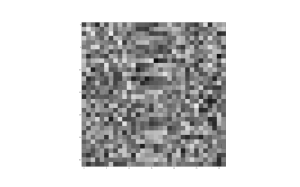
\includegraphics[scale=1]{mean-image.png}
    \end{center}
    \begin{center}
    	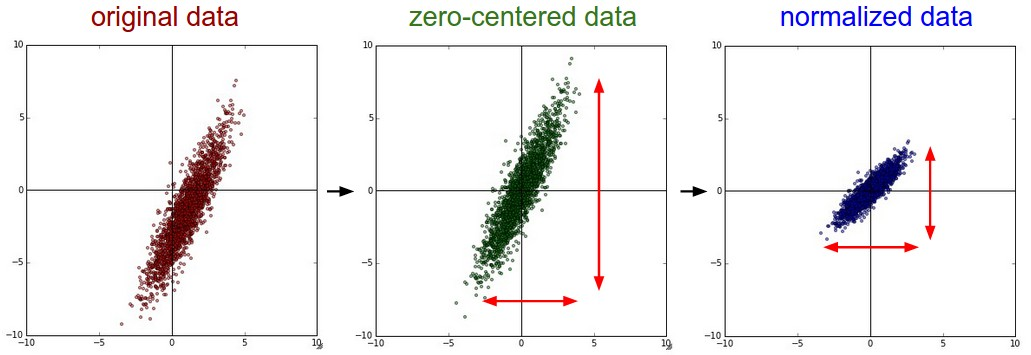
\includegraphics[scale=0.45]{zero-center.jpeg}
    	
    \end{center}
    $$\widehat{x_{i}}=\overline{x_{i}}-E_{x}\left[X\right]$$
    \subsubsection{Optymalizatory, Adam}
    
    Podczas procesu trenowania sieci zawsze dostosowujemy i zmieniamy parametry (wagi) naszego modelu, aby zminimalizować funkcję straty i uczynić nasze przewidywania możliwie poprawnymi. W tym celu używamy optymalizatorów, które aktualizują model w odpowiedzi na wynik funkcji straty.
    \\
    
    Klasycznym przykładem jest metoda gradientu, wykorzystywanego w celu zmniejszenia funkcji kosztu.
    $$w_{n+1} = w_{n} - \eta \frac{\partial}{\partial w_{n}}J(w_{n})$$
    \\
    
    Wykorzystujemy ją w programie Adaptive Moment Estimation (Adam). Jest to metoda, która oblicza adaptacyjne szybkości uczenia się dla każdego parametru. Poza przechowywaniem wykładniczo zanikającej średniej kwadratów gradientów $v_{t}$, przechowuje także wykładniczo zanikającą średnią gradientów $m_{t}$. Wartości te obliczane są ze wzorów:
    $$m_{t}=\beta_{1}m_{t-1}+\left(1-\beta_{1}\right)g_{t}$$
    $$v_{t}=\beta_{2}m_{t-1}+\left(1-\beta_{2}\right)g_{t}^2$$
    $m_{t}$ i $v_{t}$ są szacunkami odpowiednio pierwszego momentu (średniej) i drugiego momentu (wariancji niecentrowanej) gradientów. $m_{t}$ i $v_{t}$ są inicjalizowane jako wektory zerowe, stąd wartości z powyższych wzorów zbliżają się ku zeru (szczególnie, że wartości tempa rozkładu $\beta_{1}$ i $\beta_{2}$ są bliskie 1 na początku).
    \\
    
    Przeciwdziałamy tym tendencjom, obliczając szacunki pierwszego i drugiego momentu skorygowane o odchylenie:
    $$\widehat{m_{t}}=\frac{m_{t}}{1-\beta_{1}^t}$$
    $$\widehat{v_{t}}=\frac{v_{t}}{1-\beta_{2}^t}$$
    Następnie używamy tych wartości do aktualizacji parametrów, co daje regułę aktualizacji Adama:
    $$\theta_{t+1}=\theta_{t}-\frac{\eta}{\sqrt{\widehat{v_{t}}}+\epsilon}\widehat{m_{t}}$$
    
    Autorzy proponują wartości domyślne 0,9 dla $\beta_{1}$, 0,999 dla $\beta_{2}$ i 10-8 dla $\epsilon$.
    
    \subsubsection{Nvidia cuDNN}
    W naszym projekcie została użyta biblioteka \textit{tensorflow-gpu} w celu przyspieszania tworzenia modelu. Aby było to możliwe, na komputerze powinno być zainstalowane środowisko \textit{Nvidia cudNN}. W takim przypadku, model tworzy się dużo szybciej na zegarach GPU, niż CPU, jest to związane bezpośrednio z architekturą tych dwóch typów procesorów. Dzięki \textit{Nvidia cudNN} jesteśmy w stanie wykorzystać moc obliczeniową GPU. \\
    W celu wymuszenia użycia GPU zostały użyte poniższe linie kodu:
    \begin{verbatim}
    tflearn.init_graph(num_cores=4, gpu_memory_fraction=1)
    config = tf.ConfigProto()
    config.gpu_options.allow_growth = True
    session = tf.Session(config=config)
    \end{verbatim}
    
	\subsection{Implementacja}
	\subsubsection{Uproszczony schemat programu}
	\begin{center}
        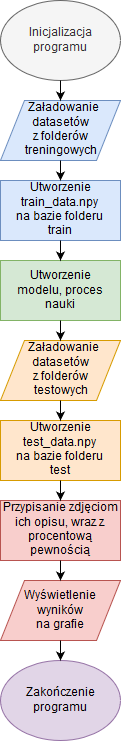
\includegraphics[scale=0.70]{schemat.png}
    \end{center}
    
    \subsubsection{Tworzenie modelu}
    Poniżej znajduję się szczegółowy opis funkcji neural\_network z pliku o tej samej nazwie, realizujący budowę modelu.
    \begin{enumerate}
        \item Następuje podział na pliki do treningu oraz walidacji, do której trafia około $10\%$ zdjęć z datasetu. Tutaj następuje także rozdzielenie macierzy w skali szarości od etykiety, która została przydzielona zdjęciu. 
        \item Wartości przechowywane wewnątrz macierzy są sprowadzane do wartości $\left[0;1\right]$. Dzieje się tak ze względu na przeprowadzenie \textit{zero-centeringu} w kolejnym kroku. Wartość, obliczana dzięki tej technice, jest używana w trakcie trenowania dla całego datasetu.
        \item Następuje budowanie modelu. Model składa się z kilku warstw:
        \begin{itemize}
            \item Warstwa konwolucji 32 filtry.
            \item Warstwa konwolucji 64 filtry.
            \item Max-pooling, stride = 2.
            \item Warstwa konwolucji 128 filtry.
            \item Max-pooling, stride = 2.
            \item Warstwa konwolucji 128 filtry.
            \item Max-pooling, stride = 2.
            \item Warstwa konwolucji 256 filtrów.
            \item Max-pooling, stride = 2.
        \end{itemize}
        W tym miejscu następuje przejście do zwykłej sieci neuronowej. Wektor 3D spłaszczany jest do wektora 1D.
        \begin{itemize}
            \item Fully-connected z 1024 neuronami, $dropout = 0.5$.
            \item Fully-connected z 1024 neuronami, $dropout = 0.5$.
            \item Wyjście z 11 neuronami.
        \end{itemize}
        \item Używamy optymalizatora Adam, funkcja straty to $categorical\_crossentropy$, określona wzorem:
        $$H(p,q)=-\sum_{x}p(x)\log_{}q(x)$$
        gdzie $p(x)$ to oczekiwane prawdopodobieństwo, $q(x)$ otrzymane prawdopodobieństwo.
        \item Następuje nauka. Do wejścia funkcji \textit{model.fit} podajemy dane do nauki, dane do walidacji, nazwę modelu, pod jaką chcemy ją zapisać, oraz \textit, czyli liczba próbek, które będą propagowane przez sieć. Im większa, tym nauka wymaga mniej pamięci. Sieć uczy się teoretycznie lepiej na mniejszych batchach, minusem natomiast tego rozwiązania jest to, że uzyskujemy mniej dokładne oszacowanie gradientu.
    \end{enumerate}
    
	\newpage
	\section{Pełen kod programu}
	\begin{itemize}
    \item Plik \textit{main.py}
	{\fontsize{9}{10}\selectfont
    	\begin{verbatim}
import numpy as np
import os
import sys
import train_data
import test_data
import neural_network1
import plot_data

class Switcher(object):
    def decision(self, argument):
        if argument.isnumeric() is False:
            sys.exit(1)
    
        if argument == "1": self.createModel()
        elif argument == "2": self.makePredictions()
        else: self.both()
    
    def createModel(self):
        if os.path.isfile('train_data.npy'):
            inp = input("Train data exist. Want to remove?")
            if inp == "yes" or inp == "y" or inp == "true":
                os.remove("train_data.npy")
                tra_data = train_data.create_train_data()
            else:
                tra_data = np.load('train_data.npy')
        else:
            tra_data = train_data.create_train_data()
    
        train_amount = len(tra_data)
        neural_network1.network1(tra_data, train_amount)
    
    def makePredictions(self):
        if os.path.isfile('test_data.npy'):
            inp = input("Test data exist. Want to remove?")
            if inp == "yes" or inp == "y" or inp == "true":
                os.remove("test_data.npy")
                tes_data = test_data.create_test_data()
            else:
                tes_data = np.load('test_data.npy')
        else:
            tes_data = test_data.create_test_data()

        plot_data.plt_dat(tes_data)
    
    def both(self):
        self.createModel()
        self.makePredictions()
    
    
if __name__ == "__main__":
    print("1. Create a model based on train dir data.")
    print("2. Make predictions based on test dir data.")
    print("3. Create a model and make preditions.")
    choice = input("Choice: ")
    
    s = Switcher()
    s.decision(choice)
    	\end{verbatim}
    }
    
    \item Plik \textit{settings.py}
	{\fontsize{9}{10}\selectfont
    	\begin{verbatim}
TRAIN_DIR = 'train'
TEST_DIR = 'test'
IMG_SIZE = 128
LR = 1e-3
MODEL_NAME = 'model.tfl'

animals = ['cat', 'dog', 'butterfly', 'chicken', 'cow', 'horse', 'lamb',
        'squirrel', 'elephant', 'spider', 'monkey']

len_animals = len(animals)

num_animals = [0 for i in range(len(animals))]
        \end{verbatim}
    }
    \item Plik \textit{train\_data.py}
	{\fontsize{9}{10}\selectfont
    	\begin{verbatim}
import cv2
import numpy as np
import os
from random import shuffle
from tqdm import tqdm
import settings as s

def create_train_data():
    training_data = []
    for animal in s.animals:
        print('Current animal:', animal, '\n')
        for img in tqdm(os.listdir(s.TRAIN_DIR + '/' + animal)):
            label = np.zeros(s.len_animals)
            label[s.animals.index(animal)] = 1
            path = os.path.join(s.TRAIN_DIR + '/' + animal, img)

            img = cv2.imread(path, cv2.IMREAD_GRAYSCALE)
            img = cv2.resize(img, (s.IMG_SIZE, s.IMG_SIZE))
            training_data.append([np.array(img), np.array(label)])

    shuffle(training_data)
    np.save('train_data.npy', training_data)
    return training_data
        \end{verbatim}
    }
    \item Plik \textit{neural\_network1.py}
	{\fontsize{9}{10}\selectfont
    	\begin{verbatim}
import numpy as np
import tensorflow as tf
import tflearn
from tflearn.layers.conv import conv_2d, max_pool_2d
from tflearn.layers.core import input_data, dropout, fully_connected
from tflearn.layers.estimator import regression
from tflearn.data_preprocessing import ImagePreprocessing
import settings as s
import os

config = tf.ConfigProto()
config.gpu_options.allow_growth = True
session = tf.Session(config=config)


def network1(train, train_amount):
    global model
    # region SPLIT DATA FOR TRAIN/VALIDATION
    train_amount = int(train_amount * 5.5 / 6)

    x_train = np.array([i[0] for i in train[:train_amount]]).reshape(-1, s.IMG_SIZE, 
                    s.IMG_SIZE, 1)
    x_train = x_train / 255.0
    y_train = [i[1] for i in train[:train_amount]]

    x_validation = np.array([i[0] for i in train[train_amount:]]).reshape(-1, s.IMG_SIZE, 
                    s.IMG_SIZE, 1)
    x_validation = x_validation / 255.0
    y_validation = [i[1] for i in train[train_amount:]]
    # endregion

    # region NETWORK
    img_prep = ImagePreprocessing()
    img_prep.add_featurewise_zero_center(mean=[0.4735053442384178])

    network = input_data(shape=[None, s.IMG_SIZE, s.IMG_SIZE, 1], name='input',
                    data_preprocessing=img_prep)

    network = conv_2d(network, 32, 3, activation='relu', scope='conv1_1')
    network = conv_2d(network, 64, 3, activation='relu', scope='conv1_2')
    network = max_pool_2d(network, 2, strides=2, name='maxpool_1')

    network = conv_2d(network, 128, 3, activation='relu', scope='conv2_1')
    network = max_pool_2d(network, 2, strides=2, name='maxpool_2')

    network = conv_2d(network, 128, 3, activation='relu', scope='conv3_1')
    network = max_pool_2d(network, 2, strides=2, name='maxpool_3')

    network = conv_2d(network, 256, 3, activation='relu', scope='conv4_1')
    network = max_pool_2d(network, 2, strides=2, name='maxpool_4')

    network = fully_connected(network, 1024, activation='relu', scope='fc5')
    network = dropout(network, 0.5, name='dropout_1')

    network = fully_connected(network, 1024, activation='relu', scope='fc6')
    network = dropout(network, 0.5, name='dropout_2')

    network = fully_connected(network, s.len_animals, activation='softmax', scope='fc7')

    network = regression(network, optimizer='adam', loss='categorical_crossentropy', 
                    learning_rate=s.LR, name='targets')

    model = tflearn.DNN(network, tensorboard_verbose=0, tensorboard_dir='log')
    # endregion

    if os.path.exists('{}.meta'.format(s.MODEL_NAME)):
        model.load(s.MODEL_NAME)
        print('Model loaded')

    # region TRAIN1
    model.fit(x_train, y_train, n_epoch=12,
              validation_set=({'input': x_validation}, {'targets': y_validation}),
              shuffle=True,
              snapshot_epoch=True,
              show_metric=True,
              batch_size=100,
              run_id=s.MODEL_NAME)
    # endregion

    # region SAVE
    model.save(s.MODEL_NAME)
    print('Network trained and saved as {0}'.format(s.MODEL_NAME))
    # endregion


        \end{verbatim}
    }
        \item Plik \textit{test\_data.py}
	{\fontsize{9}{10}\selectfont
    	\begin{verbatim}
import cv2
import numpy as np
import os
from random import shuffle
from tqdm import tqdm
import settings as s


def create_test_data():
    testing_data = []
    for img in tqdm(os.listdir(s.TEST_DIR)):
        path = os.path.join(s.TEST_DIR, img)
        img_num = img.split('.')[0]
        img = cv2.imread(path, cv2.IMREAD_GRAYSCALE)
        img_data = cv2.resize(img, (s.IMG_SIZE, s.IMG_SIZE))
        testing_data.append([np.array(img_data), img_num])

    shuffle(testing_data)
    np.save('test_data.npy', testing_data)
    return testing_data
        \end{verbatim}
    }
        \item Plik \textit{plot\_data.py}
	{\fontsize{9}{10}\selectfont
    	\begin{verbatim}
import matplotlib.pyplot as plt
import numpy as np
import settings as s
import tflearn

from tflearn.layers.conv import conv_2d, max_pool_2d
from tflearn.layers.core import input_data, dropout, fully_connected
from tflearn.layers.estimator import regression
from tflearn.data_preprocessing import ImagePreprocessing

tflearn.init_graph(num_cores=4, gpu_memory_fraction=0.5)

# region NETWORK
def cnn():
    # region NETWORK
    img_prep = ImagePreprocessing()
    img_prep.add_featurewise_zero_center(mean=[0.4735053442384178])

    network = input_data(shape=[None, s.IMG_SIZE, s.IMG_SIZE, 1], name='input',
                data_preprocessing=img_prep)

    network = conv_2d(network, 32, 3, activation='relu', scope='conv1_1')
    network = conv_2d(network, 64, 3, activation='relu', scope='conv1_2')
    network = max_pool_2d(network, 2, strides=2, name='maxpool_1')

    network = conv_2d(network, 128, 3, activation='relu', scope='conv2_1')
    network = max_pool_2d(network, 2, strides=2, name='maxpool_2')

    network = conv_2d(network, 128, 3, activation='relu', scope='conv3_1')
    network = max_pool_2d(network, 2, strides=2, name='maxpool_3')

    network = conv_2d(network, 256, 3, activation='relu', scope='conv4_1')
    network = max_pool_2d(network, 2, strides=2, name='maxpool_4')

    network = fully_connected(network, 1024, activation='relu', scope='fc5')
    network = dropout(network, 0.5, name='dropout_1')

    network = fully_connected(network, 1024, activation='relu', scope='fc6')
    network = dropout(network, 0.5, name='dropout_2')

    network = fully_connected(network, s.len_animals, activation='softmax', scope='fc7')

    network = regression(network, optimizer='adam', loss='categorical_crossentropy', 
                    learning_rate=s.LR, name='targets')

    model = tflearn.DNN(network, tensorboard_verbose=0, tensorboard_dir='log')

    model.load(s.MODEL_NAME)

    return model
# endregion


def plt_dat(test_data):
    model = cnn()
    for num in range(len(test_data)):
        d = test_data[num]
        img_data, img_num = d

        data = img_data.reshape(s.IMG_SIZE, s.IMG_SIZE, 1)
        data = data / 255.0
        prediction = model.predict([data])[0]

        s.num_animals[np.argmax(prediction)] += 1

    fig = plt.figure(figsize=(12, 8))

    for num, data in enumerate(test_data[:20]):
        img_data = data[0]

        y = fig.add_subplot(4, 5, num + 1)
        orig = img_data
        data = img_data.reshape(s.IMG_SIZE, s.IMG_SIZE, 1)
        data = data / 255.0

        model_out = model.predict([data])[0]
        str_label = '{} {:.2f}%'.format(s.animals[np.argmax(model_out)], max(model_out)*100)

        y.imshow(orig, cmap='gray')
        plt.title(str_label)
        y.axes.get_xaxis().set_visible(False)
        y.axes.get_yaxis().set_visible(False)

    for i in range(len(s.num_animals)):
        print(s.animals[i] + " : " + str(s.num_animals[i]))

    plt.show()
        \end{verbatim}
    }
    
    \end{itemize}
\end{document}

